\chapter{Revisión de técnicas}

En este capítulo se describen los procesos y algoritmos utilizados a lo largo del trabajo descrito en esta memoria. Concretamente, se comienza explicando el concepto de la \textbf{ciencia de datos} y su ciclo de vida, haciendo énfasis en \textbf{CRISP-DM} como metodología utilizada a lo largo del proyecto para resolver el problema propuesto. Tras esto, se estudian conceptos de aprendizaje automático como la \textbf{selección de modelos} o los \textbf{modelos de regresión} - haciendo especial énfasis en los modelos de \textit{ensemble} basados en técnicas de \textbf{\textit{Gradient Boosting}}


\section{Ciencia de datos y el ciclo de vida de los datos}

\subsection{Ciencia de datos}

La \textbf{ciencia de datos} es el estudio de la extracción de conocimiento útil a partir de datos, y de la generalización de dicho proceso a cualquier problema \cite{Donoho02102017}. Dicho proceso incluye la recolección y almacenamiento, mantenimiento, procesamiento, análisis y visualización de enormes cantidades de datos heterogéneos - asociados a un gran abanico de aplicaciones y dominios en muchas ocasiones multidisciplinarios \cite{10.1145/2500499}.

Desde su origen, la ciencia de datos ha evolucionado como un campo interdisciplinar que integra conocimientos y técnicas de otras disciplinas afines como el análisis de datos, la estadística o la minería de datos \cite{potential}. Ahora bien, la principal diferencia con estos campos se encuentra en el fin: el aprendizaje a partir de los datos \cite{Donoho02102017} y la capacidad de adquirir nuevo conocimiento capaz de ser utilizado para la toma de decisiones y la predicción \cite{10.1145/2500499}.

\begin{figure}[h]
	\centering
	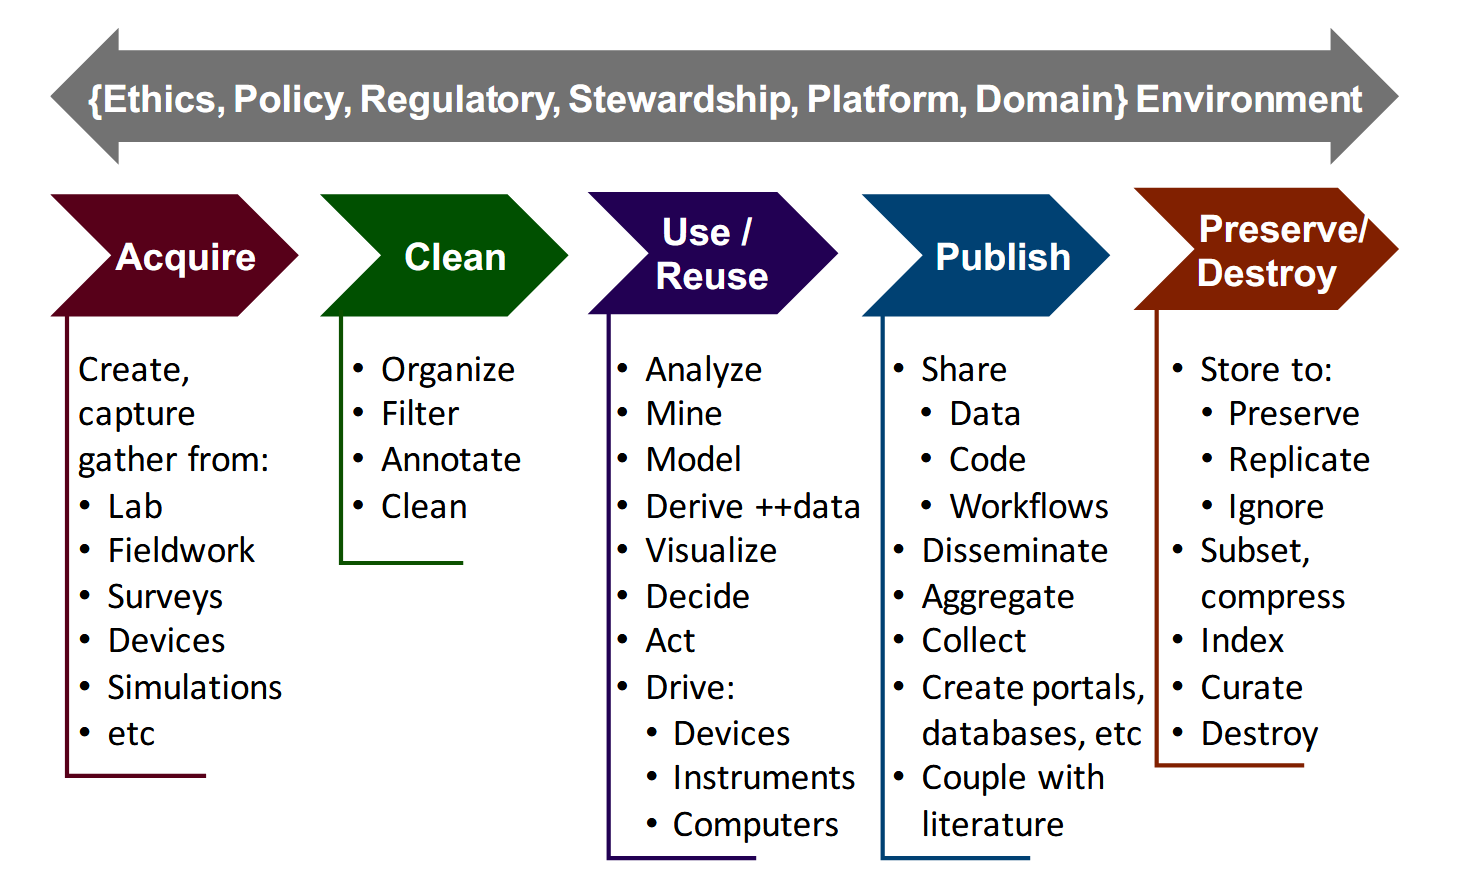
\includegraphics[width=0.8\linewidth]{figs/chapter2/datalifecycle}
	\caption{Ciclo de vida de los datos \cite{potential}}
	\label{fig:datalifecycle}
\end{figure}

Por definición, la ciencia de datos depende de los datos sobre los que se está trabajando. Por esto, el proceso de trabajo de la ciencia de datos depende generalmente del \textbf{ciclo de vida de los datos}: las distintas etapas por las que pasa un conjunto de datos desde su recolección e investigación hasta su uso final \cite{datasciencelifecycle}. Como se observa en la \textbf{Figura \ref{fig:datalifecycle}}, este ciclo está tradicionalmente dividido en \textbf{cinco} apartados \cite{potential}:



\begin{enumerate}
	\item \textbf{Adquisición:} En la actualidad, los datos se generan en cantidades masivas - del orden de \textbf{exabytes por hora} \cite{Wing2019Data}. Por tanto, el primer paso del ciclo consiste en la adquisición y almacenamiento eficiente de los datos necesarios para el proceso.
	\item \textbf{Limpieza:} Tras la adquisición, el segundo paso del ciclo consiste en la transformación de los datos originales en datos utilizables posteriormente - a través de procesos de limpieza, imputación, formateo...
	\item \textbf{Uso y re-uso:}  El tercer paso del ciclo consiste en el uso de los datos procesados con el fin de adquirir conocimiento y tomar decisiones a partir de éstos. Éste apartado se puede dividir, a su vez, en tres subapartados \cite{Wing2019Data}:
		\begin{enumerate}
			\item \textbf{Análisis exploratorio:} El estudio del comportamiento de los datos con el fin de plantear hipótesis para guiar el resto del ciclo de datos \cite{eda}.
			\item \textbf{Modelado:} El uso de técnicas computacionales y estadísticas para extraer conocimiento y predicciones a partir del conjunto de datos.
			\item \textbf{Visualización, interpretación y actuación:}  La representación gráfica de los resultados del uso de los datos, con el fin de facilitar la toma de decisiones posterior a las personas.
		\end{enumerate}
	\item \textbf{Publicación:} El cuarto paso del ciclo consiste en la diseminación de los resultados del proceso - con el fin de que el conocimiento creado pueda ser conocido y reutilizado por el mayor número de personas posible.
	\item \textbf{Preservación o destrucción:} El quinto y último paso del ciclo consiste en la preservación o destrucción de los datos utilizados - cumpliendo con otros factores como pueden ser las consideraciones éticas o regulatorias.
\end{enumerate}

Con el fin de regularizar, estandarizar y hacer reproducible el proceso completo de la ciencia de datos - desde la adquisición de los conjuntos de datos hasta la distribución de los resultados -, se han propuesto varias ampliaciones y adaptaciones del ciclo de datos estudiado, conocidas como \textbf{ciclos de vida de la ciencia de datos} \cite{datasciencelifecycle}. 

Aunque actualmente no existe un ciclo estandarizado, uno de los procesos más utilizados para ciencia de datos es el \textbf{Cross-Industry Standard Process for Data Mining (\textit{CRISP-DM})}, propuesto originalmente para el campo de la minería de datos pero adaptado a las necesidades de la ciencia de datos \cite{shearer2000crisp} - siendo el proceso utilizado a lo largo del trabajo descrito en esta memoria.

\subsection{Cross-Industry Standard Process for Data Mining - CRISP-DM}

\textbf{Cross-Industry Standard Process for Data Mining} (abreviado como \textit{CRISP-DM}) es una metodología desarrollada con el fin de ofrecer un proceso de trabajo completo de principio a fin para la minería de datos; independientemente del campo, las herramientas o la aplicación final de los datos \cite{shearer2000crisp}. Si bien fue propuesto originalmente en el año 2000, en la actualidad sigue siendo uno de los procesos más utilizados tanto en minería de datos como en ciencia de datos \cite{datasciencepmCRISPDMStill}.

\begin{figure}[h]
	\centering
	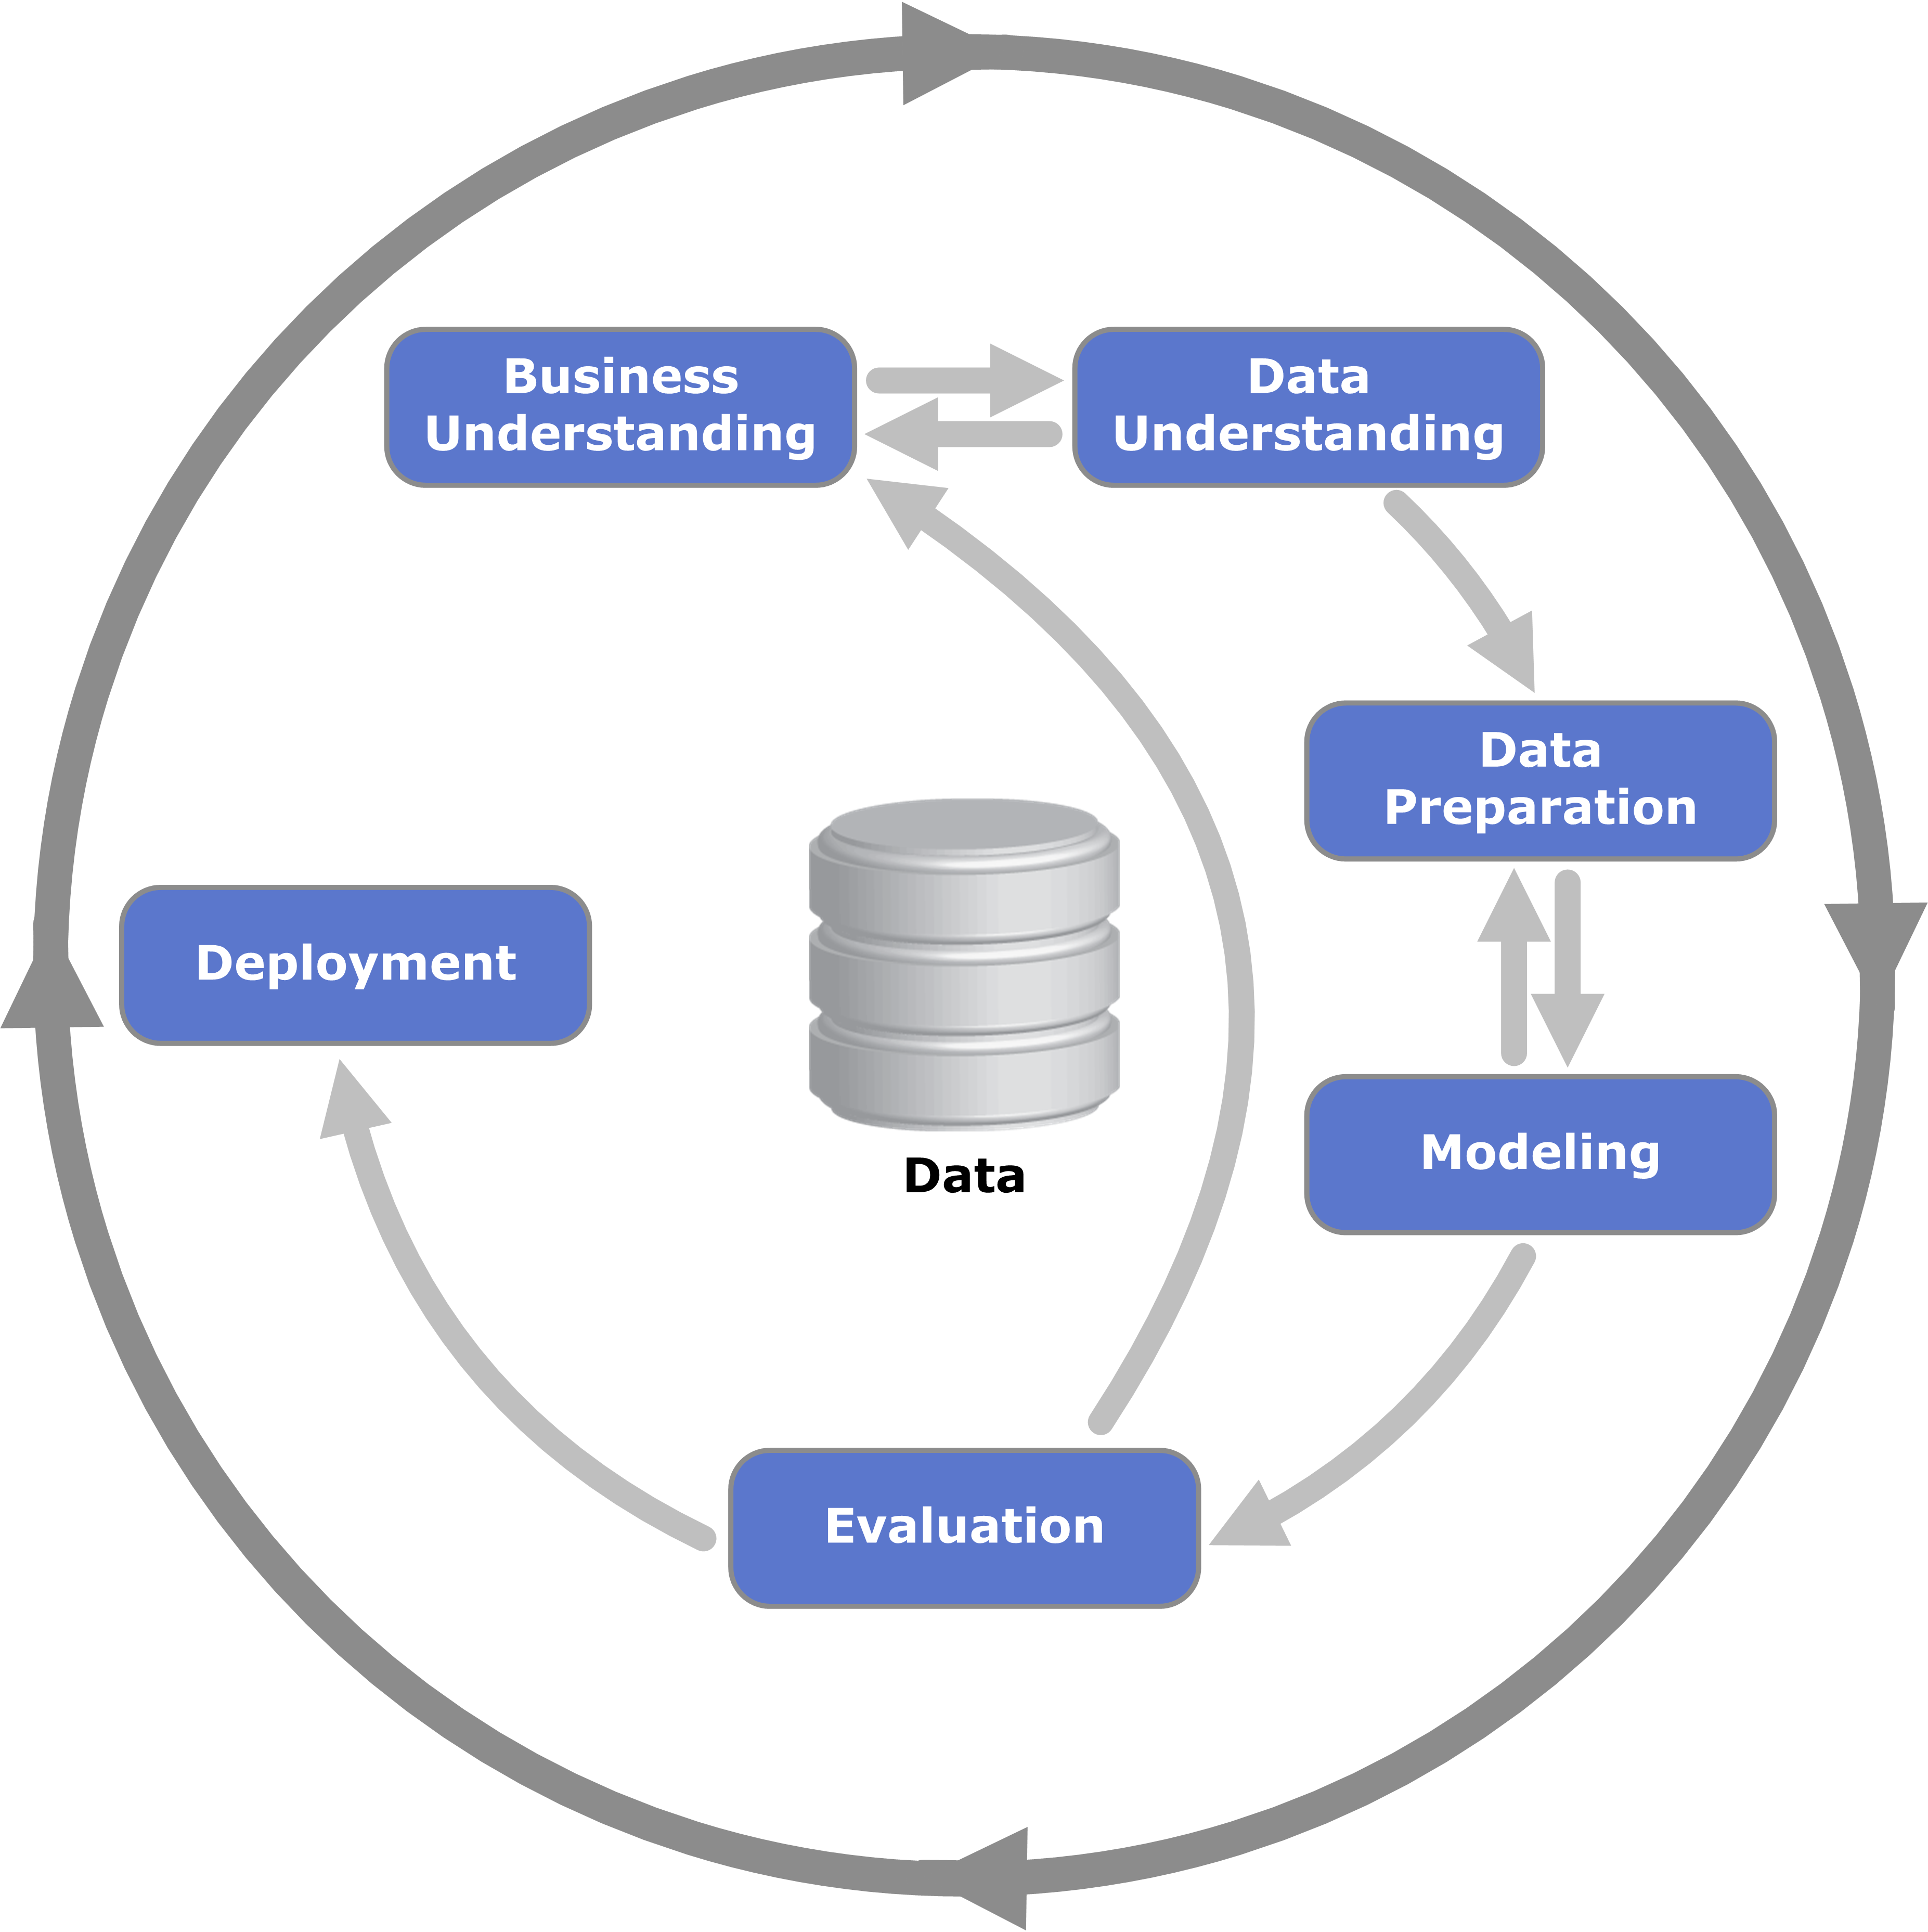
\includegraphics[width=0.6\linewidth]{figs/chapter2/crispdm}
	\caption{Ciclo de vida de CRISP-DM \cite{shearer2000crisp}}
	\label{fig:crispdm}
\end{figure}

Como se observa en la \textbf{Figura \ref{fig:crispdm}}, el ciclo de CRISP-DM está dividido en \textbf{seis fases} \cite{shearer2000crisp}, similares al ciclo de datos estudiado:

\begin{enumerate}
	\item \textbf{Conocimiento del campo (\textit{Business Understanding}):} El primer paso del ciclo consiste en entender el problema y los objetivos a resolver - estudiando la situación actual y estableciendo los pasos para alcanzar las metas propuestas.
	\item \textbf{Conocimiento de los datos (\textit{Data Understanding}):} El segundo paso del ciclo consiste en adquirir y estudiar los datos - tanto de forma superficial como en un análisis exploratorio más profundo -, además de verificar que los datos disponibles son útiles para los objetivos propuestos.
	\item \textbf{Preparación de los datos (\textit{Data Preparation}):} Tras la adquisición de conocimiento, el tercer paso consiste en preparar los datos obtenidos para su uso posterior - seleccionando las instancias relevantes, limpiando los datos para eliminar valores perdidos, enriqueciendo los datos con información externa...
	\item \textbf{Modelado (\textit{Modeling}):} Con los datos preparados, la cuarta fase del ciclo consiste en el uso y calibración de modelos de aprendizaje automático a aplicar sobre los datos - definiendo los estudios y experimentos a realizar sobre los modelos, y evaluando el rendimiento final de éstos.
	\item \textbf{Evaluación (\textit{Evaluation}):} Antes de desplegar el modelo final, la quinta fase del ciclo consiste en evaluar si los resultados obtenidos satisfacen los objetivos propuestos y si el proceso de ciencia de datos se ha aplicado de forma adecuada.
	\item \textbf{Despliegue (\textit{Deployment}):} La última fase del ciclo es el despliegue y diseminación de los resultados obtenidos - haciendo disponible el modelo y los resultados a los usuarios finales.
	
\end{enumerate}

Es importante destacar que, como indican las flechas de la \textbf{Figura \ref{fig:crispdm}}, la metodología propuesta no es linear, sino que el flujo entre los distintos pasos se puede ver alterado:
\begin{itemize}
	\item Las fases tienen dependencias entre sí - los descubrimientos en algunas fases pueden producir que sea necesario volver a fases anteriores para perfeccionar el proceso.
	\item El proceso es \textbf{cíclico} - los conocimientos adquiridos durante las distintas fases se aplican para refinar futuros procesos, ya sean sobre el mismo conjunto de datos o datos nuevos.
\end{itemize}

\section{Aprendizaje automático y ajuste de modelos}

\subsection{Aprendizaje automático}

El \textbf{aprendizaje automático} (también conocido en inglés como \textit{Machine Learning}) es una rama de la inteligencia artificial que consiste en la creación de programas capaces de \textbf{aprender} - es decir, de mejorar su rendimiento en una tarea - a través de la experiencia y de la información que se les aporta \cite{mitchell1997machine}. 

También se puede definir el término como el conjunto de métodos capaces de detectar patrones en los datos de forma autónoma, y de utilizar dichos patrones para predecir datos futuros \cite{mlprobabilistic} - siendo este último de mayor interés a los principios de la ciencia de datos.

Generalmente, los algoritmos de aprendizaje automático se dividen en dos grandes familias, en función del tipo de datos e información que se aporta a los algoritmos \cite{aima} \cite{mlprobabilistic}:

\begin{itemize}
	\item \textbf{Aprendizaje supervisado:} El objetivo del algoritmo es aprender una función capaz de, dados unos datos de entrada $X$, predecir una salida $Y$. Esta función se aprende a partir de un conjunto de datos $D={(x_i, y_i)}^{N}_{i=1}$ donde a cada instancia $x_i$ del conjunto de datos $D$ se le asocia un valor esperado $y_i$.
	
	Este tipo de aprendizaje se puede dividir a su vez en dos categorías dependiendo del tipo de salida $Y$ que se espera \cite{aima}:
	\begin{itemize}
		\item \textbf{Clasificación}: El algoritmo busca obtener para cada entrada $x_i$ un valor concreto \textbf{dentro de un conjunto finito de posibles valores}.
		\item \textbf{Regresión}: El algoritmo busca obtener, para cada entrada $x_i$, un \textbf{valor numérico continuo}.
	\end{itemize}
	\item \textbf{Aprendizaje no supervisado:} El objetivo del algoritmo es aprender patrones subyacentes de los datos de entrada $X$ ofrecidos, sin buscar predecir una salida. Esta función se aprende a partir de un conjunto de datos $D={x_i}^{N}_{i=1}$ donde no se ofrece ningún tipo de etiqueta a cada instancia $x_i$.
\end{itemize}

Un \textbf{modelo} es el resultado del proceso de aprendizaje automático: una función capaz de predecir una salida para una entrada dada, y cuyos parámetros e hiperparámetros han sido ajustados a través de un entrenamiento sobre un conjunto de datos para \textbf{minimizar un error} \cite{Burkov2019TheHM}. 

De cara a cumplir el objetivo propuesto por el trabajo descrito en esta memoria - la creación de un modelo capaz de \textbf{predecir el tiempo de diagnóstico} -, se van a trabajar con modelos supervisados de \textbf{regresión}. Por esto, resulta de interés describir los principales modelos a utilizar y el ajuste que se va a realizar sobre ellos.

\subsection{Selección de modelos}

Durante el entrenamiento de los modelos, se pueden encontrar algunos problemas:
\begin{itemize}
	\item Se han entrenado varios modelos, y es necesario elegir de forma objetiva uno de ellos en base a su rendimiento.
	\item Se necesitan elegir los hiperparámetros de un modelo que mejor rendimiento ofrecen sobre el conjunto de datos, de forma objetiva.
	\item Los modelos entrenados han aprendido variaciones insignificantes y patrones falsos - ruido interpretado como información real - a partir de los datos de entrada, llevando a un problema de \textbf{sobreajuste} \cite{mlprobabilistic} que puede afectar de forma negativa al rendimiento del modelo.
\end{itemize}

En estos casos, nos interesa seleccionar de entre todos los modelos a evaluar el modelo más \textbf{generalizable} - es decir, el modelo que tendría el \textbf{menor error esperado} si se evaluase con un conjunto de datos distinto al utilizado durante el entrenamiento \cite{mlprobabilistic}. 

Ahora bien, a la hora de la verdad no es común tener acceso a dicho hipotético conjunto de test - o si se tiene, solo debería ser utilizado para evaluar el rendimiento del modelo seleccionado finalmente para evitar que se sesgue la selección de modelos \cite{aima}. 

Para solucionar este problema y realizar una selección de modelos \textbf{honesta}, se pueden utilizar las siguientes opciones \cite{mlprobabilistic}:

\begin{itemize}
	\item \textbf{Conjunto de validación:} Se particiona el conjunto de datos inicial en entrenamiento y validación - utilizando el primero para entrenar los modelos, y el segundo para evaluar su rendimiento honesto y seleccionar el modelo.
	\item \textbf{K-Validación cruzada:} En caso de que el conjunto de datos no sea suficientemente grande para particionarse, se puede optar por particionar el conjunto de datos en \textbf{K trozos} de igual tamaño. Para cada uno de estas particiones, se entrenan los modelos con el resto de particiones y se evalúan los rendimientos sobre la partición seleccionada. Tras realizar este proceso $K$ veces, se puede utilizar el error promedio de los $K$ entrenamientos como una aproximación al rendimiento honesto del modelo para realizar la selección.
\end{itemize}

\subsection{Modelos de regresión}

En el caso de la \textbf{regresión}, el objetivo del modelo es aprender una función capaz de predecir un valor numérico continuo para cada instancia de datos de entrada \cite{mlprobabilistic}. Dicha función se ajusta buscando encontrar el conjunto de parámetros que \textbf{minimiza} la diferencia entre los valores predichos por la función y los valores reales asociados a los datos de entrada \cite{Burkov2019TheHM}.

Se han propuesto y estudiado un gran número de modelos de regresión, con parametrizaciones y funcionamientos diversos, en la bibliografía \cite{tai2021surveyregressionalgorithmsconnections}. Pese a esta variedad, es posible dividir todas estas familias de modelos en dos grandes grupos: modelos \textbf{tradicionales} y modelos de \textbf{conjuntos o \textit{ensembles}} \cite{aima}

\subsubsection{Modelos tradicionales - regresión lineal, árboles de decisiones y máquinas de vectores de soporte}

Si bien no hay una definición consensuada sobre su definición, se puede entender como \textbf{modelo tradicional} a un modelo que entrena una única función con el fin de realizar predicciones sobre la salida esperada para cada entrada de datos \cite{aima}.

Existe una gran cantidad de familias de modelos con una larga trayectoria en la bibliografía existente \cite{Burkov2019TheHM}. Ahora bien, el estudio realizado en la memoria se centra en las siguientes tres familias de modelos utilizadas en el trabajo:

\begin{itemize}[leftmargin=*]
	\item \textbf{Regresión lineal:} 
	
	Los modelos más simples, trabajando con la suposición de que \textbf{existe una correlación lineal} entre los atributos de entrada y la salida del modelo \cite{mlprobabilistic}. Por lo general, la salida $y$ para una entrada $x$ se predice utilizando la siguiente fórmula: 

	$$y(x) = \sum_{j=1}^{D}w_j x_j$$
	
	Donde $x_j$ representa cada atributo de la entrada y $w_j$ el peso asignado a cada atributo, siendo el objetivo de estos modelos ajustar los pesos asignados a cada atributo para minimizar el error cuadrado \cite{aima}. Ahora bien, cuando se trabaja con conjuntos de datos de gran dimensionalidad, el gran número de atributos puede afectar de forma negativa al rendimiento del modelo, causando un sobreajuste al conjunto de entrenamiento \cite{l1l2}.
	
	Para evitar este problema, se proponen técnicas de \textbf{regularización} - penalizaciones aplicadas a la fórmula del error con el objetivo de conseguir modelos menos complejos y más generalizables \cite{elasticnet}. Los tres modelos de regularización más utilizados son los siguientes:
	
	\begin{itemize}
		\item \textbf{Ridge (L2) \cite{ridge}:} Como factor de penalización, se utiliza $\sum_{j=1}^D(w_j)^2$ - la suma de los pesos cuadrados del modelo, buscando reducir de forma generalizada la influencia de los atributos para evitar sobreajustes y correlaciones.
		\item \textbf{Lasso (L1) \cite{lasso}:} Como factor de penalización, se utiliza $\sum_{j=1}^D|w_j|$ - la suma del valor absoluto de los pesos del modelo, buscando eliminar los atributos irrelevantes reduciendo su peso a $0$.
		\item \textbf{Elastic-Net \cite{elasticnet}:} Como factor de penalización, se utiliza $\lambda\left(\sum_{j=1}^D(w_j)^2\right) + (1-\lambda)\left(\sum_{j=1}^D|w_j|\right)$ - utilizando a la vez las regularizaciones L1 y L2 de forma ponderada, buscando aunar los beneficios de ambas aproximaciones.
	\end{itemize}

	\item \textbf{Máquinas de vectores de soporte (SVM):} 
	
	Las máquinas de vectores de soporte se pueden entender como una evolución de los modelos de regresión lineal donde, en vez de buscar la linea que mejor se ajusta al conjunto de datos, se busca el \textbf{hiperplano} capaz de ajustarse al conjunto de datos con el \textbf{mayor margen} \cite{aima}. 
	
	En regresión, esto se traduce en la búsqueda de la función representando al mejor hiperplano capaz de ajustarse a todas las instancias del conjunto de datos a la vez que es capaz de mantener una distancia inferior a un margen $\epsilon$ con todos los puntos \cite{svr}.
	
	La principal utilidad de estos modelos radica en las dos siguientes características \cite{aima}:
	\begin{itemize}
		\item \textbf{Funciones kernel:} Un problema de los modelos lineales es que los conjuntos de datos no siempre son linealmente separables. Para solventar este problema, las máquinas de vectores de soporte son capaces de utilizar \textbf{funciones \textit{kernel}} para transformar los datos a una mayor dimensionalidad - donde si es posible ajustar un hiperplano con mayor margen.
		\item \textbf{Vectores de soporte:} Para definir el modelo no es necesario almacenar información sobre el conjunto de datos completo, sino que es suficiente con almacenar información sobre los \textbf{puntos que definen la frontera entre el hiperplano y el margen} - conocidos como los vectores de soporte.
	\end{itemize}
	\newpage
	\item \textbf{Árboles de decisión:} 
	
	Los árboles de decisión son modelos de reglas representando su función a través de grafos dirigidos \cite{Burkov2019TheHM} donde la predicción se obtiene realizando una serie de comprobaciones secuenciales empezando desde la raíz, ramificando hasta llegar a una hoja final \cite{aima}. Estos árboles se dividen en los siguientes componentes:
	
	\begin{itemize}
		\item \textbf{Nodos:} Nodos internos del árbol donde se realiza una comprobación sobre el valor de un atributo. Dependiendo del resultado de la comprobación, el nodo se \textbf{ramifica} a otros nodos u hojas.
		\item \textbf{Hojas:} El valor final predicho para una entrada, alcanzado tras una serie de comprobaciones en nodos.
	\end{itemize}
	
	El objetivo del modelo es, por tanto, aprender el conjunto de reglas que minimiza el error del modelo para el conjunto de datos dado. Ahora bien, estos modelos tienden a \textbf{sobreajustar} creando árboles de gran profundidad \cite{aima}.

\end{itemize}

\subsubsection{Modelos de ensemble - bagging y boosting}

Como contraste a los modelos tradicionales, un \textbf{modelo de conjunto, meta-modelo o \textit{ensemble}} es un modelo que, durante su entrenamiento, ha aprendido un \textbf{conjunto de funciones o modelos sencillos} - por lo general, una agrupación de modelos tradicionales -, agrupando las predicciones de todos éstos para obtener una predicción general de la salida esperada para cada entrada de datos \cite{aima}.

Los algoritmos de \textit{ensemble} buscan aprender un gran número de modelos simples con rendimiento ligeramente mejor que un modelo aleatorio - conocidos como \textbf{modelos de aprendizaje débil}, generalmente \textbf{árboles de decisión} \cite{Burkov2019TheHM}. Suponiendo que cada uno de estos modelos es completamente independiente al resto, la unión de sus resultados lleva a una predicción final \textbf{más precisa y generalizable} que un único modelo entrenado \cite{Burkov2019TheHM}.

Dependiendo de la metodología utilizada para entrenar los modelos simples - ya sea de forma secuencial o paralela -, se pueden dividir los algoritmos en dos familias \cite{aima}:


\begin{itemize}[leftmargin=*]

	\item \textbf{Bootstrap Aggregating (Bagging):} 
	
	Los modelos de \textit{ensemble} trabajan con la suposición de que cada uno de los modelos individuales que lo componen es totalmente independiente al resto de modelos. Ahora bien, en la práctica no suele ser factible entrenar a cada modelo individual sobre un conjunto de datos independiente \cite{baggingart}. 
	
	Para solventar este problema, los modelos de \textbf{\textit{bagging}} entrenan cada modelo sobre una \textbf{muestra uniformemente aleatoria con reemplazo} (\textit{bootstrap} en inglés) del conjunto de datos original \cite{baggingart} - obteniendo como resultados modelos sencillos e independientes, y siendo la predicción final el \textbf{promedio} de las predicciones de cada modelo.

	Algunos de los modelos de \textit{bagging} más importantes son los siguientes:
	
	\begin{itemize}
		\item \textbf{\textit{Random Forest} \cite{randomforests}:} Un modelo de \textit{ensemble bagging} de \textbf{árboles de decisión profundos} en el que se añade un segundo proceso de muestreo aleatorio para aumentar la independencia entre los predictores simples entrenados:
		\begin{itemize}
			\item \textbf{Muestreo de instancias:} Cada árbol se entrena con un subconjunto aleatorio de instancias del conjunto de datos.
			\item \textbf{Muestreo de atributos:} Cada árbol se entrena con un subconjunto aleatorio de atributos del conjunto de datos.
		\end{itemize}
		\item \textbf{\textit{Extremely Randomized Trees \cite{Geurts2006}:}} Una evolución del modelo de \textit{Random Forest} en el que se añade un proceso de muestreo adicional, con los siguientes cambios:
		\begin{itemize}
			\item Cada árbol pasa a entrenarse sobre el \textbf{conjunto de datos completo}, sin muestreo - aunque se sigue realizando un muestreo de los atributos a considerar por cada árbol.
			\item Durante la construcción del árbol, se generan de forma aleatoria varias \textbf{particiones del conjunto de datos} para cada atributo - en vez de calcular la partición óptima. A la hora de construir cada nodo, se elige la partición que mejor puntuación obtiene de todas las generadas.
		\end{itemize}
	\end{itemize}
	
	\item \textbf{Boosting:}
	
	Para garantizar la independencia entre los modelos entrenados, los modelos de \textit{ensemble} de tipo \textbf{boosting} optan por entrenar sus modelos de forma \textbf{secuencial} sobre un \textbf{conjunto de datos con pesos} - donde, para cada modelo, se da más peso a las instancias del conjunto de datos que se han predicho erróneamente en los modelos anteriores \cite{aima}.
	
	Durante el trabajo, se ha considerado el siguiente modelo de \textit{boosting}:
	
	\begin{itemize}
		\item \textbf{\textit{Adaptive Boosting \cite{adaboost}:}} Un modelo básico de \textit{boosting} que sigue estrictamente el proceso descrito. Concretamente, se comienza con un conjunto de datos de pesos uniformes sobre el que se entrena el primer modelo, ajustando los pesos de las instancias - aumentando el peso de las instancias con mayor error, y reduciendo el peso de las instancias con menor error. Tras esto, se repite el proceso de entrenamiento de modelos y ajuste de pesos hasta entrenar todos los predictores \cite{aima}.
		
		La predicción final es una \textbf{media ponderada por el error} de la predicción de todos los modelos - donde los modelos con menor error tienen un mayor peso en la ponderación.
	\end{itemize}
	
	Una subfamilia dentro de estos algoritmos son los modelos de \textbf{Gradient Boosting}. Estos modelos también utilizan la metodología de \textit{boosting} - entrenar modelos secuencialmente ajustándose a los errores del modelo anterior -, con la diferencia de que el entrenamiento no se hace sobre el conjunto de datos directamente, sino sobre los \textbf{errores residuales} (la diferencia entre la predicción y el valor real) de cada instancia \cite{gradientboosting}. 
	
	Este comportamiento es similar al \textbf{gradiente descendiente} utilizado para entrenar otros modelos como la regresión lineal o las redes neuronales \cite{Burkov2019TheHM}. En concreto, se llevan a cabo los siguientes pasos:
	\begin{enumerate}
		\item Se comienza realizando una predicción inicial, generalmente el valor promedio de todas las instancias.
		\item Utilizando el valor estimado, se calculan los \textbf{errores pseudo-residuales} de cada instancia - el \textbf{error} entre la predicción y el valor real. Estas pseudo-residuales dependen de la función de error que se elija.
		\item Repitiéndose para cada modelo que se tiene que entrenar:
		\begin{enumerate}
			\item A partir de los valores pseudo-residuales, se entrena un modelo simple que \textbf{predice el valor residual de cada instancia}.
			\item Utilizando los nuevos residuales estimados, se recalculan los valores pseudo-residuales para que el siguiente modelo ajuste mejor a las instancias clasificadas erroneamente.
		\end{enumerate}
	\end{enumerate}
	
	Para obtener una predicción final, se suma al valor promedio inicial los residuales calculados por cada uno de los modelos - ponderados por un \textbf{factor de aprendizaje} para evitar el sobreajuste \cite{gradientboosting}.
	
	Actualmente, los modelos de \textit{Gradient Boosting} son considerados el estado del arte para la mayoría de problemas de predicción estructurada \cite{Burkov2019TheHM}, siendo algunos de los modelos más populares los siguientes:
	
	\begin{itemize}
		\item \textbf{\textit{Extreme Gradient Boosting \cite{Chen_2016}:}} Un algoritmo de \textit{Gradient Boosting} utilizando el método de Newton-Raphson - en vez de calcular los errores pseudo-residuales, se calcula una función de la segunda y la primera derivada de la función de error. Además, el modelo está diseñado para permitir el entrenamiento en paralelo de los árboles.
		\item \textbf{\textit{Categorical Boosting \cite{dorogush2018catboostgradientboostingcategorical}:}} Un algoritmo de \textit{Gradient Boosting} diseñado para trabajar de forma nativa con atributos categóricos sin necesidad de convertirlos previamente a valores numéricos. 
		
		El modelo se entrena utilizando \textbf{\textit{Ordered Boosting}} - utilizando una permutación aleatoria del conjunto de entrenamiento para cada modelo, donde para calcular las pseudo-residuales de cada instancia se consideran solo las instancias anteriores en la permutación \cite{catboost2} - para evitar introducir sesgos.
		\item \textbf{\textit{Light Gradient-Boosting Model \cite{NIPS2017_6449f44a}:}} Un algoritmo de \textit{Gradient Boosting} con las siguientes características:
		\begin{itemize}
			\item \textbf{Histogramas:} Para optimizar el rendimiento, los valores de los atributos continuos se agrupan en histogramas.
			\item \textbf{Crecimiento del arbol por hojas:} Frente a otros algoritmos que entrenan los árboles nivel a nivel, el modelo ramifica siempre por la hoja que minimizaría el error - llevando a árboles más ajustados.
		\end{itemize}
		
		Existe otra implementación de este algoritmo, conocida como \textbf{Histogram-Based Gradient Boosting}, ofrecida por la librería de ciencia de datos \textit{Scikit-Learn} \cite{scikit-learn} - aunque ambas se basan en el mismo modelo y no presentan diferencias significativas.
	\end{itemize}
\end{itemize}

